% topic4.tex -- Module 8 Topic 4: Properties of the nucleus, Q43-56.
\topictitle{Topic 4 - Properties of the Nucleus}

% ---- Q43 (alpha, beta, gamma in an electric field)
% P = beta (strongly towards +), Q = gamma (straight), R = alpha (slightly towards -)
\begin{quizq}{}
A radioactive source emits alpha, beta and gamma radiation into the space between two charged parallel
plates. The paths P, Q and R are shown.
\begin{center}
  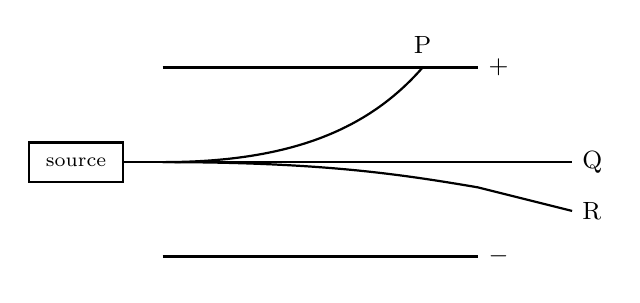
\begin{tikzpicture}
    \draw[line width=1.3pt] (0,1.2) -- (4,1.2) node[right, font=\small] {$+$};
    \draw[line width=1.3pt] (0,-1.2) -- (4,-1.2) node[right, font=\small] {$-$};
    \draw[line width=0.8pt] (-1.7,-0.25) rectangle (-0.5,0.25); \node[font=\scriptsize] at (-1.1,0) {source};
    \draw[line width=0.8pt] (-0.5,0) -- (0,0);
    \draw[line width=0.8pt] (0,0) .. controls (1.6,0) and (2.6,0.4) .. (3.3,1.2); \node[above, font=\small] at (3.3,1.25) {P};
    \draw[line width=0.8pt] (0,0) -- (5.2,0) node[right, font=\small] {Q};
    \draw[line width=0.8pt] (0,0) .. controls (2,0) and (3,-0.15) .. (4,-0.32) -- (5.2,-0.62) node[right, font=\small] {R};
  \end{tikzpicture}
\end{center}
Which row correctly identifies the paths?
\begin{center}
  \renewcommand\arraystretch{1.7}
  \begin{tabular}{@{}p{10mm}|>{\centering\arraybackslash}p{28mm}|>{\centering\arraybackslash}p{28mm}|>{\centering\arraybackslash}p{28mm}|}
    \cline{2-4}
    & \textit{Alpha} & \textit{Beta} & \textit{Gamma}\\ \cline{2-4}
    A. & P & Q & R\\ \cline{2-4}
    B. & P & R & Q\\ \cline{2-4}
    C. & R & P & Q\\ \cline{2-4}
    D. & Q & R & P\\ \cline{2-4}
  \end{tabular}
\end{center}
\end{quizq}

% ---- Q44 (neutron absorption then alpha decay)
\Needspace{14\baselineskip}
\begin{quizq}{}
A nucleus absorbs a neutron. The new nucleus then emits an alpha particle, leaving a lithium-7 nucleus
(\nuc{7}{3}{Li}). What was the original nucleus?
\opts{\nuc{7}{4}{Be}}{\nuc{11}{5}{B}}{\nuc{12}{6}{C}}{\nuc{10}{5}{B}}
\end{quizq}

% ---- Q45 (alpha decay product)
\Needspace{12\baselineskip}
\begin{quizq}{}
Radium-226 (\nuc{226}{88}{Ra}) undergoes alpha decay. What is the daughter nucleus?
\opts{\nuc{222}{86}{Rn}}{\nuc{226}{86}{Rn}}{\nuc{222}{88}{Ra}}{\nuc{230}{90}{Th}}
\end{quizq}

% ---- Q46 (beta-minus decay equation)
\Needspace{14\baselineskip}
\begin{quizq}{}
Which equation correctly shows the beta-minus decay of carbon-14?
\opts{$\nuc{14}{6}{C} \rightarrow \nuc{14}{5}{B} + \nuc{0}{+1}{e} + \nu$}
  {$\nuc{14}{6}{C} \rightarrow \nuc{14}{7}{N} + \nuc{0}{-1}{e} + \bar{\nu}$}
  {$\nuc{14}{6}{C} \rightarrow \nuc{10}{4}{Be} + \nuc{4}{2}{He}$}
  {$\nuc{14}{6}{C} \rightarrow \nuc{13}{6}{C} + \nuc{1}{0}{n}$}
\end{quizq}

% ---- Q47 (decay on a neutron-proton chart)
% X at N = 144, Z = 90; Y at N = 143, Z = 91 (beta-minus)
\Needspace{34\baselineskip}
\begin{quizq}{}
The chart shows part of a neutron--proton chart. Nucleus X decays into nucleus Y, as shown by the arrow.
\begin{center}
  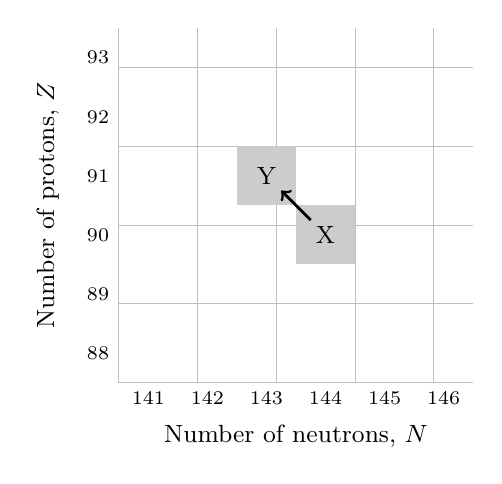
\begin{tikzpicture}[x=0.75cm, y=0.75cm]
    \draw[black!25, line width=0.4pt] (0,0) grid (6,6);
    \foreach \i/\n in {0/141,1/142,2/143,3/144,4/145,5/146} \node[below, font=\scriptsize] at (\i+0.5,0) {\n};
    \foreach \j/\z in {0/88,1/89,2/90,3/91,4/92,5/93} \node[left, font=\scriptsize] at (0,\j+0.5) {\z};
    \node[below, font=\small] at (3,-0.55) {Number of neutrons, $N$};
    \node[rotate=90, font=\small] at (-1.2,3) {Number of protons, $Z$};
    \fill[black!20] (3,2) rectangle (4,3); \node[font=\small] at (3.5,2.5) {X};
    \fill[black!20] (2,3) rectangle (3,4); \node[font=\small] at (2.5,3.5) {Y};
    \draw[->, line width=1pt] (3.25,2.75) -- (2.75,3.25);
  \end{tikzpicture}
\end{center}
What type of decay is shown?
\opts{Alpha decay}{Beta-plus decay}{Beta-minus decay}{Gamma decay}
\end{quizq}

% ---- Q48 (mass left after three half-lives)
\Needspace{12\baselineskip}
\begin{quizq}{}
A sample contains \qty{80}{g} of a radioactive isotope. What mass of the isotope remains after three
half-lives?
\opts{\qty{40}{g}}{\qty{26.7}{g}}{\qty{20}{g}}{\qty{10}{g}}
\end{quizq}

% ---- Q49 (parent : daughter after two half-lives)
\Needspace{12\baselineskip}
\begin{quizq}{}
A rock contained a radioactive isotope but none of its stable daughter isotope when it formed. What is the
ratio of parent atoms to daughter atoms after two half-lives?
\opts{1 : 4}{1 : 3}{1 : 2}{1 : 1}
\end{quizq}

% ---- Q50 (decay constant from a graph)
\Needspace{32\baselineskip}
\begin{quizq}{}
The graph shows how the mass of a radioactive isotope in a sample changes with time.
\begin{center}
  \begin{tikzpicture}[x=0.4cm, y=0.1cm]
    \draw[black!20, line width=0.3pt, xstep=2, ystep=5] (0,0) grid (16,40);
    \draw[axisline] (0,0) -- (17,0) node[right, font=\small] {Time (days)};
    \draw[axisline] (0,0) -- (0,44) node[above, font=\small] {Mass (g)};
    \foreach \x in {0,4,...,16} \node[below, font=\scriptsize] at (\x,0) {\x};
    \foreach \y in {10,20,30,40} \node[left, font=\scriptsize] at (0,\y) {\y};
    \draw[line width=1pt, domain=0:16, samples=60, smooth] plot (\x, {40*2^(-\x/4)});
  \end{tikzpicture}
\end{center}
What is the decay constant of the isotope?
\opts{\qty{0.17}{day^{-1}}}{\qty{0.25}{day^{-1}}}{\qty{2.8}{day^{-1}}}{\qty{4.0}{day^{-1}}}
\end{quizq}

% ---- Q51 (activity graphs: smallest decay constant)
% A: half-life 3 h; B: straight line reaching A0/2 at 2 h; C: half-life 1 h; D: half-life 2 h (0.3 cm per hour)
\Needspace{34\baselineskip}
\begin{quizq}{}
Which graph shows the activity $A$ of a radioactive sample against time $t$ for the isotope with the
SMALLEST decay constant? All four samples start with the same activity $A_0$.
\gridopts{%
  \begin{tikzpicture}\gaxesP{$A$}{$t$ (h)}
    \draw[guide] (0,0.75) -- (2.5,0.75); \node[left, font=\scriptsize] at (0,0.75) {$\frac{A_0}{2}$}; \node[left, font=\scriptsize] at (0,1.5) {$A_0$};
    \foreach \x/\l in {0.6/2, 1.2/4, 1.8/6, 2.4/8} \node[below, font=\scriptsize] at (\x,0) {\l};
    \draw[line width=1pt, domain=0:2.5, samples=50, smooth] plot (\x, {1.5*2^(-\x/0.9)});
  \end{tikzpicture}}
  {%
  \begin{tikzpicture}\gaxesP{$A$}{$t$ (h)}
    \draw[guide] (0,0.75) -- (2.5,0.75); \node[left, font=\scriptsize] at (0,0.75) {$\frac{A_0}{2}$}; \node[left, font=\scriptsize] at (0,1.5) {$A_0$};
    \foreach \x/\l in {0.6/2, 1.2/4, 1.8/6, 2.4/8} \node[below, font=\scriptsize] at (\x,0) {\l};
    \draw[line width=1pt] (0,1.5) -- (1.2,0);
  \end{tikzpicture}}
  {%
  \begin{tikzpicture}\gaxesP{$A$}{$t$ (h)}
    \draw[guide] (0,0.75) -- (2.5,0.75); \node[left, font=\scriptsize] at (0,0.75) {$\frac{A_0}{2}$}; \node[left, font=\scriptsize] at (0,1.5) {$A_0$};
    \foreach \x/\l in {0.6/2, 1.2/4, 1.8/6, 2.4/8} \node[below, font=\scriptsize] at (\x,0) {\l};
    \draw[line width=1pt, domain=0:2.5, samples=50, smooth] plot (\x, {1.5*2^(-\x/0.3)});
  \end{tikzpicture}}
  {%
  \begin{tikzpicture}\gaxesP{$A$}{$t$ (h)}
    \draw[guide] (0,0.75) -- (2.5,0.75); \node[left, font=\scriptsize] at (0,0.75) {$\frac{A_0}{2}$}; \node[left, font=\scriptsize] at (0,1.5) {$A_0$};
    \foreach \x/\l in {0.6/2, 1.2/4, 1.8/6, 2.4/8} \node[below, font=\scriptsize] at (\x,0) {\l};
    \draw[line width=1pt, domain=0:2.5, samples=50, smooth] plot (\x, {1.5*2^(-\x/0.6)});
  \end{tikzpicture}}
\end{quizq}

% ---- Q52 (activity after 10 days)
\Needspace{12\baselineskip}
\begin{quizq}{}
Iodine-131 has a half-life of 8.0 days. A sample has an activity of \qty{800}{Bq}. What is its activity
10 days later?
\opts{\qty{1.0e2}{Bq}}{\qty{2.3e2}{Bq}}{\qty{3.0e2}{Bq}}{\qty{3.4e2}{Bq}}
\end{quizq}

% ---- Q53 (binding energy of helium-4)
\Needspace{14\baselineskip}
\begin{quizq}{}
The mass of a helium-4 nucleus is \qty{4.001506}{u}. The mass of a proton is \qty{1.007276}{u} and the
mass of a neutron is \qty{1.008665}{u}. What is the binding energy of the helium-4 nucleus?
\opts{\qty{0.0304}{MeV}}{\qty{7.07}{MeV}}{\qty{28.3}{MeV}}{\qty{3.73e3}{MeV}}
\end{quizq}

% ---- Q54 (what a larger total binding energy means)
\Needspace{14\baselineskip}
\begin{quizq}{}
Nucleus X has a larger total binding energy than nucleus Y. Which statement MUST be true?
\opts{X has a greater mass than Y.}{X has a larger mass defect than Y.}{X is more stable than Y.}
  {X has more protons than Y.}
\end{quizq}

% ---- Q55 (energy from binding energies)
\Needspace{16\baselineskip}
\begin{quizq}{}
The binding energies of three nuclei are: \nuc{2}{1}{H}, \qty{2.22}{MeV}; \nuc{3}{1}{H}, \qty{8.48}{MeV};
\nuc{4}{2}{He}, \qty{28.30}{MeV}. How much energy is released in this fusion reaction?
\[ \nuc{2}{1}{H} + \nuc{3}{1}{H} \rightarrow \nuc{4}{2}{He} + \nuc{1}{0}{n} \]
\opts{\qty{39.0}{MeV}}{\qty{28.3}{MeV}}{\qty{17.6}{MeV}}{\qty{6.26}{MeV}}
\end{quizq}

% ---- Q56 (the moderator in a fission reactor)
\Needspace{16\baselineskip}
\begin{quizq}{}
What is the function of the moderator in a nuclear fission reactor?
\opts{It slows down neutrons, so that they are more likely to cause fission of uranium-235 nuclei.}
  {It absorbs neutrons, so that the chain reaction can be stopped.}
  {It carries heat away from the core to make steam.}
  {It shields workers from gamma radiation.}
\end{quizq}
